\section{Ejercicio 8}

\begin{figure}[h]
	\centering                                                       
	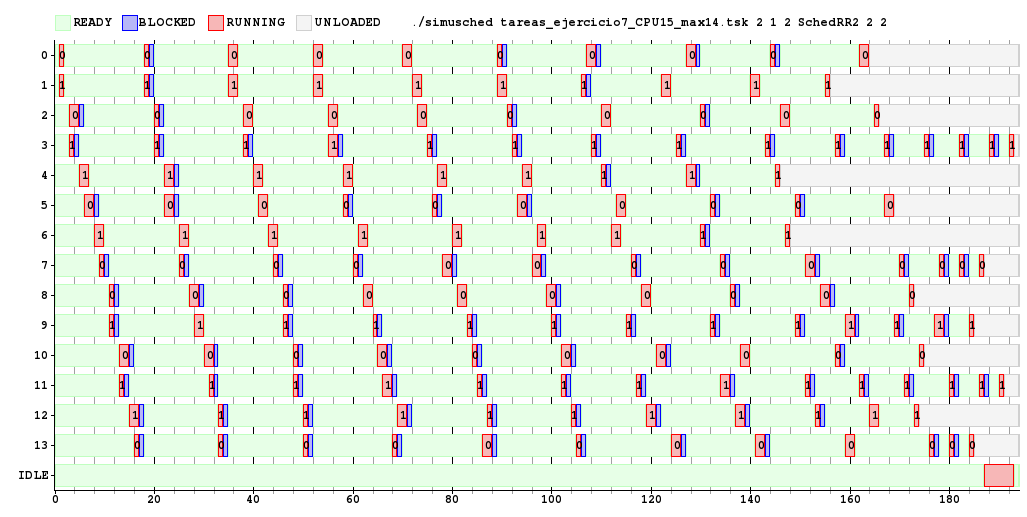
\includegraphics[width=450pt]{./figs/ejercicio8_2cores_quantum2.png}
\end{figure}

Lo que podemos ver al comparar la implementación de \textit{Round Robin 2} a diferencia del ejercicio 7, es que tenemos un algoritmo que no permite la migración de un proceso de un core a otro. Esto trae aparejado tanto ventajas como desventajas. En el primer grupo tenemos la ausencia del costo de migración entre núcleos, porque, lógicamente, dicha penalización no existe. En nuestras pruebas (con los costos de cambio de core y contexto fijados por el enunciado), esta ventaja es evidente cuando el quantum es pequeño, ya que la migración representa un porcentaje más alto de tiempo ``perdido'', en relación a la duración de cada turno para cada tarea. En nuestra experimentación en particular, se puede ver en el ejemplo de 2 cores, que baja el \textit{turnaround time} de aproximadamente 264 ticks a  198.\\
\indent Por otro lado, cuando el quantum no es pequeño, y los procesadores se utilizan de mejor forma, las tareas terminan de ejecutarse antes. Esto hace que la cantidad de veces que se cambia el núcleo de ejecución sean menos, haciendo que si eliminamos ese costo, no estemos mejorando de una manera tan importante el resultado final de la ejecución (es decir, estamos quitando algo que por otras características del experimento, ya no es tan protagonista de las mediciones como antes) como veremos a continuación.

\begin{figure}[h]
	\centering                                                       
	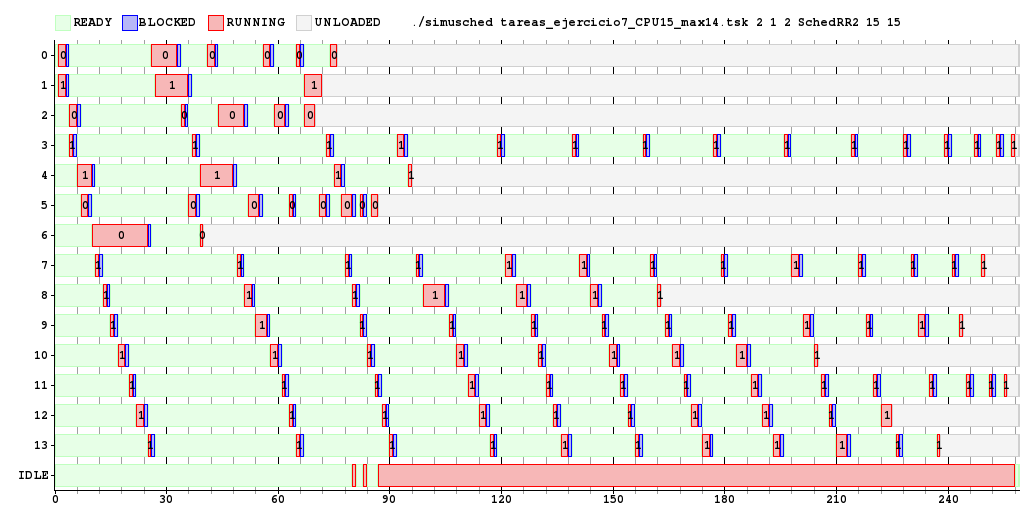
\includegraphics[width=450pt]{./figs/ejercicio8_2cores_quantum15.png}
\end{figure}

\clearpage

Las mejoras dadas por la falta de costo de migración de core no están presentes en el \textit{turnaround time}. No solo eso, sino que por el contrario, el \textit{turnaround time} es peor que en la experimentación con los mismos parámetros, pero con el algoritmo usado en el ejercicio 7.\\
\indent Esto es porque, como dijimos, no se aprovecha la fijación de una tarea con un core. El mayor problema con este enfoque es que uno no sabe de antemano cuanto va a tardar una tarea en terminar, y puede ser que mientras una tarea termina rápido, otra esté en estado \textit{ready}, atada a otro core, esperando su turno, mientras hay otro/s CPU/s en estado idle. Esto hace que el porcentaje de \textit{CPU Utilization} con este escenario disminuya de forma alarmante. Un CPU en estado idle existiendo tareas en estado \textit{ready} es una de las peores cosas que le pueden pasar a un algoritmo de scheduling como los que estamos viendo en este trabajo.